\section{Stakeholder analysis}\label{sec:stakeholders}

\begin{center}
\textquote[\footnotemark]{\textit{A stakeholder is a party that has an interest in a company, and can either affect or be affected by the business.}}
\end{center}
% 
\footnotetext{\url{http://www.investopedia.com/terms/s/stakeholder.asp}, accessed 09-05-2017}
% 
When starting (having) a business, it is important to analyse who your stakeholders are. It is because they may have an affect on your business in one way or another. In the field of platooning we have defined several of them. It starts with truck manufacturers as developers, continues with shippers (companies whose goods is being shipped), carriers (companies that are shipping goods) and truck drivers as users and then government and regulators. Citizens/other drivers are also affected by platooning as it has impact traffic as whole. Each of them have different power and interest in the platooning and therefore they have been put in the chart below.\par
% 
\begin{figure}[h]
    \centering
    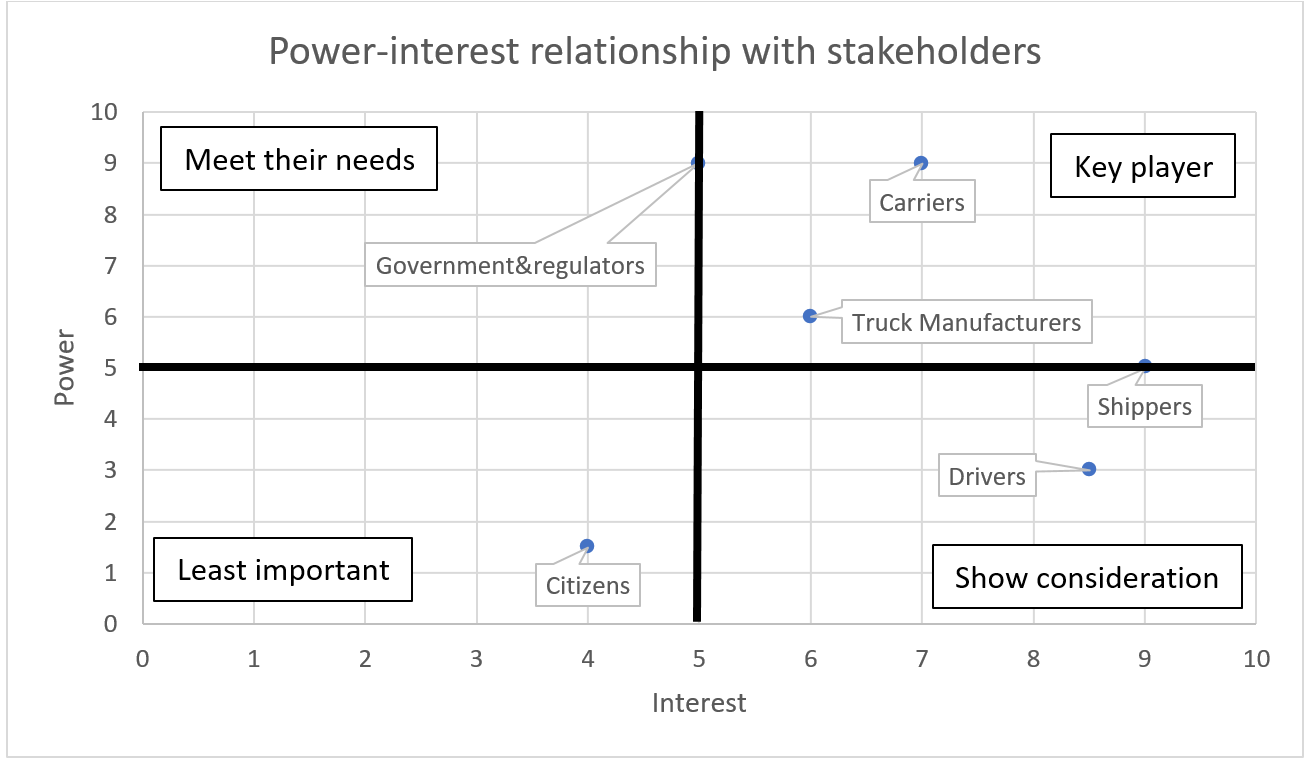
\includegraphics[width=.95\textwidth]{stakeholder-chart}
    \caption{Approximate placement of the stakeholders on the power-interest chart.}
    \label{fig:stakeholder-chart}
\end{figure}
% 
As it can be seen in Figure \ref{fig:stakeholder-chart}, there are different entities with different views. That may cause hard time in fulfilling needs and will of all of them as they may be many times in opposition. But lets break it down and look at every stakeholders’ needs separately.\par
% 
\subsection{Shippers}
Are companies/customers that would like to transport goods from point A to B. They are not direct users of platooning and do not have any extra costs when launching the technology of platooning they only can save money. This may eventually create the pressure from shippers on carrier companies to use the technology, because everyone in the business wants to lower its cost if possible. Therefore, they have kind of big power in beginnings of platooning and may “force” carrier to adapt the technology.
% 
% 
\par \textbf{Main motivation:} Save money for the transport of products, reducing the risk of products being damaged in crash and building ECO image of the brand (see \hyperref[sec:data]{Chapter} \ref{sec:data} for details).
%
\par \textbf{Biggest obstacle:} Trust in technology has to be established.
% 
% 
\subsection{Carriers}
Companies that are transporting goods. They are the ones bearing the additional costs of trucks (technology) and so they will have a big influence in adapting the technology and its future success. It is up to them to adapt the technology (unless there is a law) and cooperate with each other. This may cause problem between competing companies in the business as they may refuse to share/establish a platoon (this is only supposition). Smaller freight companies are more likely to adapt the technology by "jumping into bandwagon" (bandwagon effect) meaning that the more platooning vehicles are on road, the more likely they will join.
% 
\par \textbf{Main motivation:} Save money on fuel, safety of truck drivers(see \hyperref[sec:data]{Chapter} \ref{sec:data}). Companies adapting this technology first will have the advantage of being the first and "future ready" as well as it may help them in building better image of the company. Being first on the market does not necessary mean advantage over competition because of not enough platooning truck on the road.
% 
\par \textbf{Biggest obstacle:} Higher initial cost of a truck, cooperation between transport companies.
% 
\subsection{Truck manufacturers}
Nowadays, in the technically advanced world, new technologies are being developed constantly. It cannot be doubted that a company that comes up with a new technology and bring it successfully to the market has a big market advantage, because it can offer something that its competitors cannot at that moment. Therefore, big truck companies like Volvo, Scania, etc. are trying to develop their solutions for platooning and are doing technology push to the market and seize the opportunity of being first. They are also taking part in projects like SARTRE \cite{Chan2012ProjectSARTRE} or Companion \cite{2016CompanionProject} which helps them with gathering crucial data for future development. However, this non-cooperative development and being first hunting, leads to the development of systems that are not usually compatible within different brands.\par
% 
\par \textbf{Main motivation:} By introducing the technology first, get a market share and earn more in sales \cite{Banbury1995TheSurvival}.\par
% 
\par \textbf{Biggest obstacle:} Non-existing regulations and no global standard (system architecture) for platooning, resulting in incompatible systems from different manufacturers.\par
% 
\subsection{Drivers}
% 
They are the ones, that will be benefiting from the technology the most as during their drive, they may be resting, eating or do some other work not connected to driving. Therefore, they would be fresher, once they take over the drive again, which may lead to lower crash rate. On the other hand, freight companies may lower salaries to drivers as they would not be basically working while platooning or they may be assigned additional work to do while on the road. Platooning may also solve the possible future shortage of truck drivers \cite{OMarah2016TruckImagination} because of unmanned trucks in platoon.\par
% 
\par \textbf{Main motivation:} Possibility of rest during a drive and safety \cite[p. 37]{Chan2012ProjectSARTRE}.\par
% 
\par \textbf{Biggest obstacle:} Drivers may be afraid of new technology and having the truck "out of control" \cite{Sadeghian2016CooperativePrototype}. Also, they may be requested to other work while not driving or earn less.\par
% 
\subsection{Government and regulators}
% 
Government and regulatory authorities play a big role in the process of adaptation of the platooning. By passing laws in favour of platooning the government may help to popularise it among people and speed up its entrance on the market (tax-reliefs, etc.) It is also beneficial for the state to have platooning vehicles on roads as this will save it money, by bigger safety on road and less need of building new/bigger roads. Regulators however, should set regulations strictly enough to have platooning safe, but on the other hand these regulations should not be barriers for platooning.
% 
\par \textbf{Main motivation:} Saving money on infrastructure (building roads) and hospital charges as safety is higher\cite[p. 37]{Chan2012ProjectSARTRE}.
% 
\par \textbf{Biggest obstacle:} Infrastructure (side road units) may need to be built.\par
% 
\subsection{Citizens and other drivers}
% 
Ordinary people is the last and biggest group of stakeholders in our analysis. They do not have big power over platooning but they are affected by it.
% 
\par \textbf{Main motivation:} Possible saving of money on products, safety and less congestion (see \hyperref[sec:data]{Chapter} \ref{sec:data}).\par
% 
\par \textbf{Biggest obstacle:} Afraid of autonomous trucks on platoon.\par
% 
After having the stakeholder analysis done, we identified our stakeholders which are Carriers, Shippers, Government and regulators, truck drivers, truck manufacturers and other people. We also identified the needs of these stakeholder groups their interests and power. This will help us to derive some requirements from this as well as we will know with which stakeholders we should be cooperating with.